% XGBoost v4 Ablation Study — Component Criticality
% Replaces: tab:xgboost-v4-ablation in section_xgboost_v4_ridge.tex
% Horizontal bar chart showing degradation when components are removed

\begin{figure}[htbp]
\centering
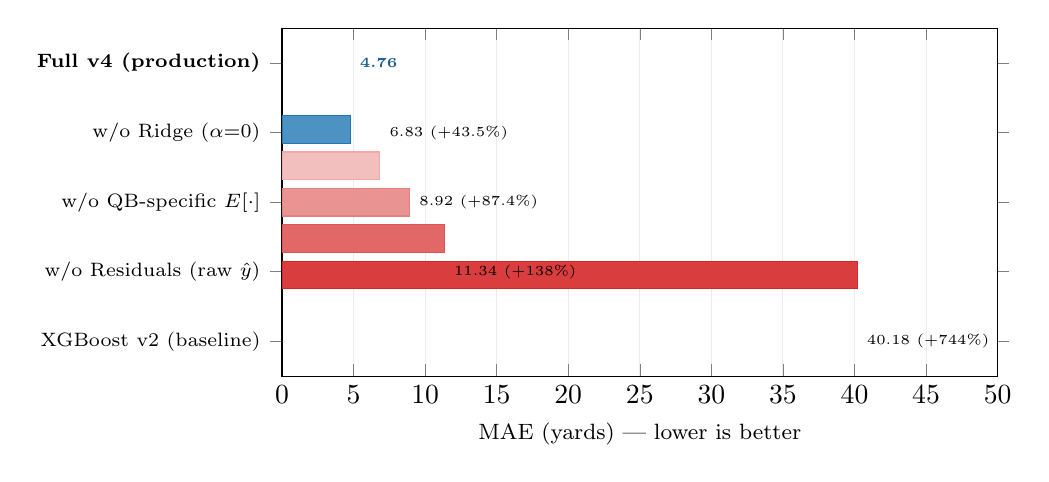
\begin{tikzpicture}
\definecolor{accent}{RGB}{31,119,180}
\definecolor{accentRed}{RGB}{214,39,40}

\begin{axis}[
  width=0.88\textwidth,
  height=6cm,
  xbar,
  bar width=10pt,
  xmin=0, xmax=50,
  xlabel={MAE (yards) --- lower is better},
  xlabel style={font=\footnotesize},
  ytick={1,2,3,4,5},
  yticklabels={
    {\textbf{Full v4 (production)}},
    {w/o Ridge ($\alpha{=}0$)},
    {w/o QB-specific $\mathbb{E}[\cdot]$},
    {w/o Residuals (raw $\hat{y}$)},
    {XGBoost v2 (baseline)}
  },
  yticklabel style={font=\scriptsize},
  y dir=reverse,
  grid=major,
  grid style={gray!15},
  xmajorgrids=true,
  ymajorgrids=false,
  enlarge y limits={abs=0.5},
]

% Full v4 (highlighted)
\addplot[fill=accent!80, draw=accent] coordinates {(4.76, 1)};

% Ablation variants (increasingly red)
\addplot[fill=accentRed!30, draw=accentRed!40] coordinates {(6.83, 2)};
\addplot[fill=accentRed!50, draw=accentRed!60] coordinates {(8.92, 3)};
\addplot[fill=accentRed!70, draw=accentRed!80] coordinates {(11.34, 4)};
\addplot[fill=accentRed!90, draw=accentRed] coordinates {(40.18, 5)};

% Value labels
\node[font=\tiny\bfseries, anchor=west, text=accent!80!black] at (axis cs:4.76,1) {4.76};
\node[font=\tiny, anchor=west] at (axis cs:6.83,2) {6.83 (+43.5\%)};
\node[font=\tiny, anchor=west] at (axis cs:8.92,3) {8.92 (+87.4\%)};
\node[font=\tiny, anchor=west] at (axis cs:11.34,4) {11.34 (+138\%)};
\node[font=\tiny, anchor=west] at (axis cs:40.18,5) {40.18 (+744\%)};

\end{axis}
\end{tikzpicture}
\caption[XGBoost v4 ablation]{XGBoost v4 component ablation (2023 holdout, 148 games). Removing any component causes severe degradation: ridge regularization prevents overfitting (+43.5\% MAE without), QB-specific centering breaks residual correlation (+87.4\%), and ensemble residual signal is irreplaceable (+138\%). The v2 baseline (no ensemble signal) shows the full 744\% gap.}
\label{fig:xgb-v4-ablation-chart}
\end{figure}
